\section{Physical Represenatations}
\label{sec:physical}

We considered three in-memory \tg representations that differ in
compactness, but also, perhaps more importantly, in the kind of
locality they prioritize. With {\em structural locality}, neighboring
vertices of the same snapshot are laid out together, while with {\em
  temporal locality}, consecutive states of the same vertex are laid
out together.  SnapshotGraph (SG), a representation in which each
snapshot is stored explicitly, naturally preserves structural
locality, but temporal locality is lost. OneGraph (OG) stores all
vertices and edges of an evolving graph once, in a single data
structure.  This representation emphasizes temporal locality, while
also preserving structural locality.  HybridGraph (HG) trades
compactness for better structural locality, by aggregating together
several consecutive snapshots, and computing a OneGraph for each
snapshot cluster.

{\bf SnapshotGraph (SG).} The simplest way to represent an evolving
graph is by representing each snapshot individually, a direct
translation of our logical data model.  We call this data structure
SnapshotGraph, or SG for short. An example of an SG is depicted in
Figure~\ref{fig:sgp}.  SG is a collection of snapshots, where vertices
and edges store the attribute values for the specific time interval.
A \insql{TSelect} operation on this representation is a slice of the
snapshot sequence, while \insql{TGroup} and temporal joins
(\insql{TAnd} and \insql{TOr}) require a group by key within each
aggregate set of vertices and edges.

\begin{figure}[t!]
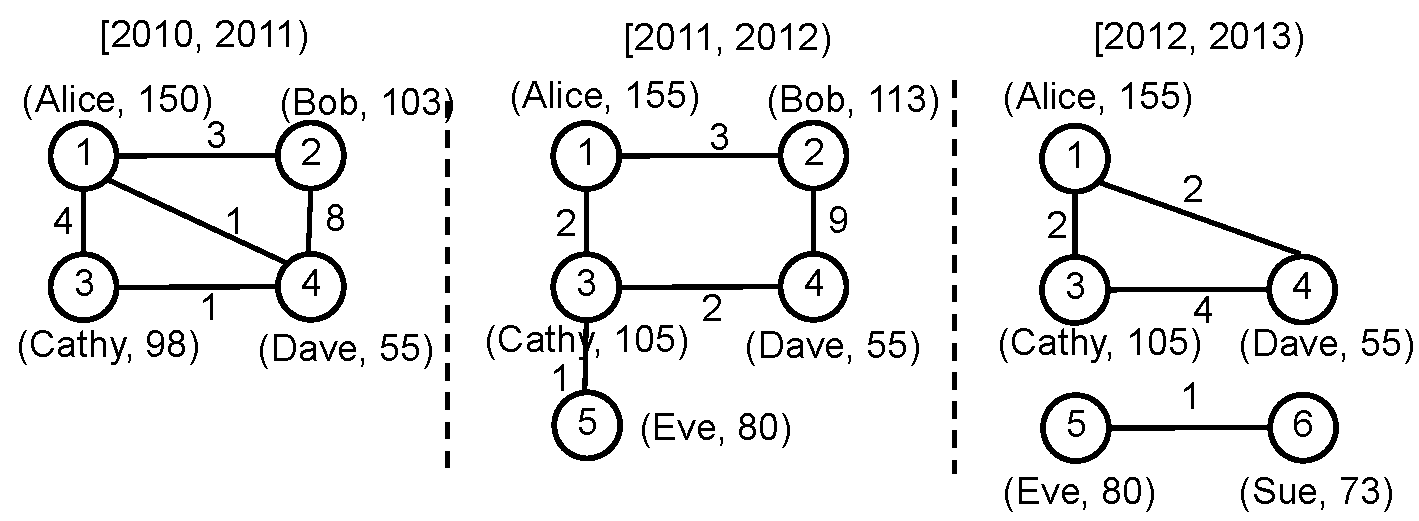
\includegraphics[width=3.3in]{figs/sgp.pdf}
\caption{SG representation of T1 from Figure~\ref{fig:tg_t1}.}
\label{fig:sgp}
\vspace{-0.3cm}
\end{figure}

While the SG representation is simple, it is not compact, considering
that in many real-world evolving graphs there is a 80\% or larger
similarity between consecutive
snapshots~\cite{DBLP:journals/tos/MiaoHLWYZPCC15}.  In a distributed
architecture, however, this data structure provides some benefits as
operations on it can be easily parallelized, by assigning different
snapshots to different workers, or by partitioning a snapshot across
workers.  

{\bf OneGraph (OG).}  The most topologically compact representation of
graph structure is to store each vertex {\em and} each edge only once
for the whole evolving graph, by taking a union of the snapshot vertex
and edge sets.  The OneGraph data structure, or OG for short, uses
this representation in our system.  The drawback is that OG is much
denser than individual snapshots of SG.  OG stores vertex and edge
attribute information separately.  This is not as compact as storing
attributes within the graph elements, but is faster in many operations
where only graph topology is required.

\begin{figure}[t!]
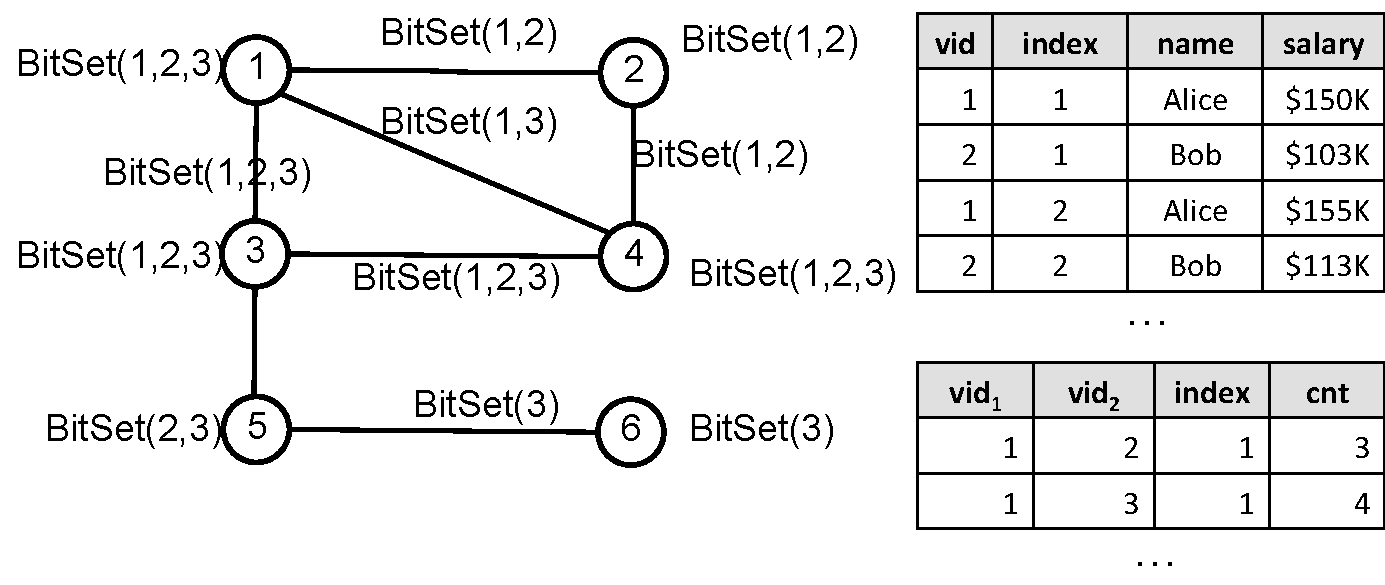
\includegraphics[width=3.2in]{figs/ogc.pdf}
\vspace{-0.3cm}
\caption{OG representation of T1 from~\ref{fig:tg_t1}.}
\vspace{-0.5cm}
\label{fig:ogc}
\end{figure}

{\bf HybridGraph (HG).} As an intermediate representation between SG
and OG, we implement the HybridGraph (HG) data structure.  HG is a
series of OGs, with each OG representing some number of temporally
adjacent snapshots.

In our current implementation each OG in the sequence corresponds to
the same number of temporally adjacent snapshots.  This is the
simplest snapshot clustering method, yet, as we will see in
Section~\ref{sec:exp}, it already improves performance
compared to OG.  However, we also observed that placing the same
number of snapshots into each cluster often results in unbalanced
cluster sizes.  This is because networks commonly exhibit strong
temporal skew, with later snapshots being significantly larger than
earlier ones.  Consequently, we are currently working on more
sophisticated clustering approaches that would lead to better balance,
and ultimately to better performance.

{\bf Partitioning strategies.}  Graph partitioning can have a
tremendous impact on system performance.  A good partitioning strategy
needs to (1) be balanced, assigning an approximately equal number of
units to each partition, and (2) limit the number of cuts across
partitions, to reduce cross-partition communication.

There are two basic types of graph partitioning strategies. Vertex-cut
(also known as edge partitioning) distributes edges across the
available machines and replicates vertices as necessary, while
edge-cut (vertex partitioning) does the opposite.  Vertex-cut
approaches have been shown to have better
performance~\cite{Gonzalez2012}, and are the strategies of choice in
GraphX.  \ql leverages these strategies.

In our experiments we compare performance of SG, OG and HG with (1) no
repartitioning after load, and (2) with repartitioning using the 2D
edge partitioning strategy (E2D).  This strategy is available in
GraphX and was used without modification.  In E2D, a sparse edge
adjacency matrix is partitioned in two dimensions, guaranteeing a $2
\sqrt{n}$ bound on vertex replication, where $n$ is the number of
partitions. As we will see in Section~\ref{sec:exp}, E2D provides good
performance for Pregel-style analytics.

We implemented and are experimenting with additional partitioning
strategies as part of our ongoing work.
